
We formally state the problem and performance measures.
\vspace{-0.6em}

\subsection{Online Data Stream}
\label{subsec:online_data_stream}

A data-stream of length $T \in \mathbb{N}$ is a collection of $T$, independent, scalar valued random variables $(S_t)_{t=1}^T$, indexed by time $t \in [T]$ \footnote{For any positive integer $L$, we denote $[L] = \{1,\cdots,L\}$}. In practice, $S_t \in \mathbb{R}$ at time $t$ is the \emph{anomaly score} of an input sample produced by an AD algorithm such that high scores corresponds to anomalies.
For each time $t \in [T]$,  $f_t$ is the probability distribution of $S_t$, i.e., $S_t \sim f_t$. We assume $f_t$ is a continuous measure without discrete atoms.\footnote{Formally, $\forall p \in (0,1)$, the set $\{ Q \in \mathbb{R}: \mathbb{P}_{X \sim f}[X \leq Q] = p\}$ has exactly one element.} Since the distribution $f_t$ is indexed by time $t$, $(S_t)_{t=1}^T$ is not necessarily identically distributed and thus non-stationary. We assume that the data-stream although is non-stationary, is piece-wise stationary. 

\begin{definition}(Piece-wise stationary) Let $T$ be the time horizon and let $H_T \leq T-1$ be the total number of change points. Define a set of strictly increasing time indices  $1 < \tau_1 < \tau_2 \cdots < \tau_{H_T}$ as change points; let $\tau_0 = 0$ and $ \tau_{H_T+1} = T$. A piece-wise stationary data-stream $(S_t)_{t=1}^T\sim\Bigl(T,H_T, (\tau_c)_{c=0}^{H_T}, (f^{(c)})_{c=0}^{H_T}\Bigr)$ is such that $\forall k \in [1, H_T]$:
\begin{itemize}[noitemsep,topsep=-2pt,labelwidth=!, labelindent=0pt]
   \item $\forall t \in [\tau_k,\tau_{k+1})$, $S_t \sim f^{(k)}$ are i.i.d. with the $p$-quantile of $f^{(k)}$ denoted as $ Q^{(k)}(p) \in \mathbb{R}$. %Thus, $\forall t \in [\tau_k,\tau_{k+1})$, 
    \item  $f^{(k)} \neq f^{(k+1)}$
\end{itemize}
\label{def:piecewise}
\end{definition}

\begin{figure}[h!]
    \centering
    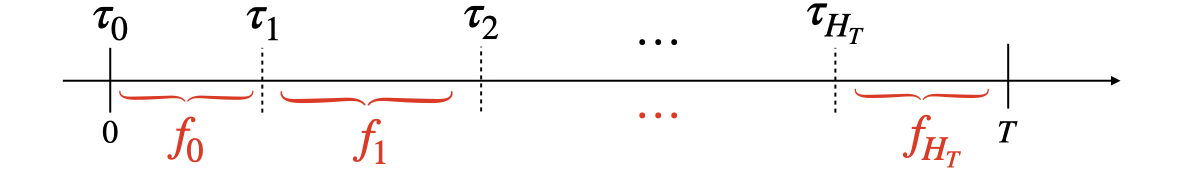
\includegraphics[width=0.9\linewidth]{anomaly/figs/piecewise.jpeg}
    \caption{The piece-wise stationary process}
    \label{fig:enter-label}
    \vspace{-0.8em}
\end{figure}

The special case of $H_T = 0$ corresponds to a stationary i.i.d. data stream.
We remark that our algorithm does not have any information on the change-points  $H_T$, $(\tau_t)_{t=1}^{H_T}$, nor on distributions $(f^{(c)})_{c=0}^{H_T}$. %Nevertheless, the performance  of our algorithm will adapt with the complexity of the data-stream. 

\subsection{Anomaly Definition} 
\label{subsec:anomaly_defn}
%
%As is standard, anomalies are as those time points where the observed sample $S_t$ is larger than the $p$th quantile.
%Following convention \cite{chandola2009anomaly}, we will assume that large values of scores are anomalies. 

\begin{definition}[Anomalies] 
The sample $S_t \sim f_t$ at time $t$ is an anomaly if $S_t > \tau_t$, where $\tau_{t} = \inf \{ \tau\geq 0: \mathbb{P}_{S \sim f_t}[S \leq \tau] \geq p \}$ and $p \in (0,1)$. We denote by $y_t = \mathbf{1}(S_t > \tau_t)$ the indicator variable that the sample $S_t$ is an anomaly.
% \begin{align}
% \begin{split}
%    y_t &= \mathbf{1}(X_t > \tau_{p} ), \text{where} \\
%     \tau_{p} &= \inf \{ \tau\geq 0: \mathbb{P}_{X_t \sim f_t}[X_t \leq \tau] \geq p \}
% \end{split} 
% \end{align} 
\label{def:anomaly}
\end{definition}
%\vspace{-1em}
In words, a sample $S_t$ is anomalous if it exceeds the threshold $\tau_t$ corresponding to the $p$th quantile. Thus, the thresholding algorithm needs to estimate $\tau_t$ and then use that estimate to make the binary decision of whether $S_t$ is an anomaly.
We assume the quantile value $p \in (0,1)$ to be known. 
%In practice, knowledge of $p$ arises, either from constraints on the rate of anomalies that can be investigated \cite{hassan2019nodoze, ho2021hopper}, or from domain knowledge on the base rate of anomalies \cite{perini2023unsupervised}.
% and is thus an extrinsic input.  %While this paper is motivated by anomaly detection and thus focuses on extreme values on one side, but our definitions and algorithms can easily be modified to detect anomaly on both sides, by simultaneously estimating a low and a high quantile.

\subsection{Offline Datasets}
\label{subsec:offline_datasets}

We formalize the notion of \emph{offline datasets} that can be used in addition to using historical samples on the data-stream. Offline datasets are typically available to train the anomaly scoring systems \cite{bhatia2022memstream, audibert2020usad} and have been used to address the cold-start problem in previous works \cite{gutflaish2019temporal,hofmann1999probabilistic}.


 \begin{definition}[Offline Dataset] We define an offline dataset as $K$ sets of independent samples $\mathcal{D} := \{\{X_i^{(j)}\}_{i=1}^{N_j} \}_{j=1}^K$. Each $j \in \{1,\cdots,K\}$ set $\{X_i^{(j)}\}_{i=1}^{N_j}$  are independent samples such that all of the $N_j$ samples are drawn from distributions having the same $p$th quantile denoted by $Q_{(j)}(p)$. A special case is $\{X_i^{(j)}\}_{i=1}^{N_j}$ are i.i.d., with all $N_j$ samples having identical distributions and thus identical $p$th quantile.
 \label{definition:offline_dataset}
 \end{definition}

Observe that $\mathcal{D} = \emptyset$ corresponds to the special case of no offline data availabe.
We will assume that $K$, the number of partitions are known to the algorithm. Clustered offline datasets is a valid assumption, since typically, the offline data is pre-processed before deploying online algorithms. In practice, the clusters could correspond to different groups of signals, e.g. different sensor types, different environmental conditions or day of the week \cite{khan2020industrial, audibert2020usad, sadik2014research}. 

\subsection{Online Anomaly Thresholding Algorithm}
\label{subsec:oad_algo_defn}
 
\begin{definition} An online anomaly thresholding algorithm $\gA$ outputs a label  $\hat{y}_t = \mathcal{A} (S_t; (S_1, \ldots,S_{t-1}), \mathcal{D})\in \{0,1,* (\text{abstain})\}$, a decision for the score $S_t$ depending on the history $S_1, \cdots, S_{t-1}$ and offline datasets $\mathcal{D}$ if any. 
\label{def:algo}
\end{definition}

We emphasize the dependence on the offline dataset $\mathcal{D}$ in the algorithm since that can be used to make a decision at all times. 
However, as mentioned before, the algorithm has no information about the data-stream quadruple, nor any parametric information on the distribution from which either the scores $(S_t)_{t=1}^T$ or the offline dataset $\mathcal{D}$ are sampled from. 
% Since we are interested in assessing the online performance, we make this assumption that the offline dataset is perfectly clustered. We defer the effect of imperfections in the offline data on the online performance to the future.

% \begin{itemize}
%     \item No assumptions on underlying distributions, i.e., $f_t \in \mathcal{M}$ for all $t$.
%     \item small number of mistakes (false positives and false negatives), sub-linear growth of abstains.    
%     \item The performance guarantees are adaptive to small number of distribution shifts in the stream.
%     \item In the presence of a offline dataset: If the test stream is similar to the dataset, then we want to leverage the past and yield improved results. 
%     \item  If the test online stream is arbitrary, then we do not want the online performance to be arbitrarily bad - rather it should be comparable to standard online algorithms that does not assume prior knowledge. 
% \end{itemize}

\subsection{Performance Measures}
\label{subsec:performance_defnition}

The three performance measures of an anomaly thresholding algorithm are {\em (i)} False Positives $\text{FP} = \sum_{t=1}^T \mathbf{1}(\hat{y}_1 = 1, y_t = 0)$, {\em (ii) } False Negatives $ \text{FN} = \sum_{t=1}^T \mathbf{1}(\hat{y}_0 = 1, y_t = 1)$, and {\em (iii)} $\text{Abstains} = \sum_{t=1}^T \mathbf{1}(\hat{y}_t = *)$. We
denote by $\text{Mistakes} := \text{FP} + \text{FN}$ as the sum of false-positives and negatives. The desiderata of high-accuracy and low abstains translate to having a constant independent of $T$ mistakes and a sub-linear in $T$ abstains. 